\section{Your First Program}
\label{sec:first_program}

\subsection{While Loops}
\label{sub:while_loops}
\begin{frame}[fragile]
	\frametitle{While Loops}
	\begin{lstlisting}[keepspaces=true]
		while(conditional) {
		  // Code to execute when true
		}
	\end{lstlisting}
	While loops executes the code contained within them while their conditional statement is true.
	\begin{block}{Example}
		A main function should (almost) never exit:
		\begin{lstlisting}[keepspaces=true]
			int main() {
			  while(true) {
			    // Main loop code, runs forever
			  }
			}
		\end{lstlisting}
	\end{block}
\end{frame}

\begin{frame}
	\frametitle{Your Program}
	\begin{columns}[c]
		\begin{column}{0.5\textwidth}
			\lstinputlisting[caption=main.cpp]{code/first_program/1.cpp}
		\end{column}
		\begin{column}{0.5\textwidth}
			\begin{itemize}
				\item Add an infinite while loop to your main function to prevent your program from ending.
			\end{itemize}
		\end{column}
	\end{columns}
\end{frame}

\subsection{Digital Output}
\label{sub:digital_output}
\begin{frame}[fragile]
	\frametitle{Digital Output}
	DigitalOut constructor:
	\begin{lstlisting}[numbers=none]
		DigitalOut(PinName pin)
	\end{lstlisting}
	It creates an object attached to the given pin. Anytime you see PinName, use a name from the images on the next slide.
	
	You can assign a value to the object using the equals sign. 1 turns the pin on while a 0 turns the pin off.
	\begin{block}{Example}
		Attach a DigitalOut to the LED1 pin on the Nucleo and turn it on:
		\begin{lstlisting}[numbers=none]
			DigitalOut led(LED1);
			led = 1;
		\end{lstlisting}
	\end{block}
\end{frame}

\begin{frame}
	\frametitle{Nucleo Pin Names}
	\begin{columns}[c]
		\begin{column}{0.5\textwidth}
			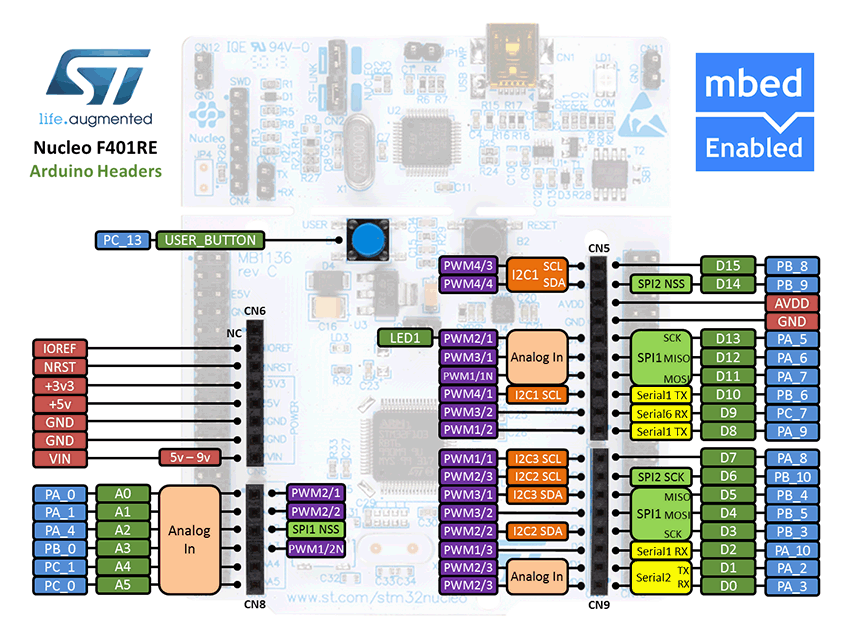
\includegraphics[width=\linewidth]{arduino_pins}
		\end{column}
		\begin{column}{0.5\textwidth}
			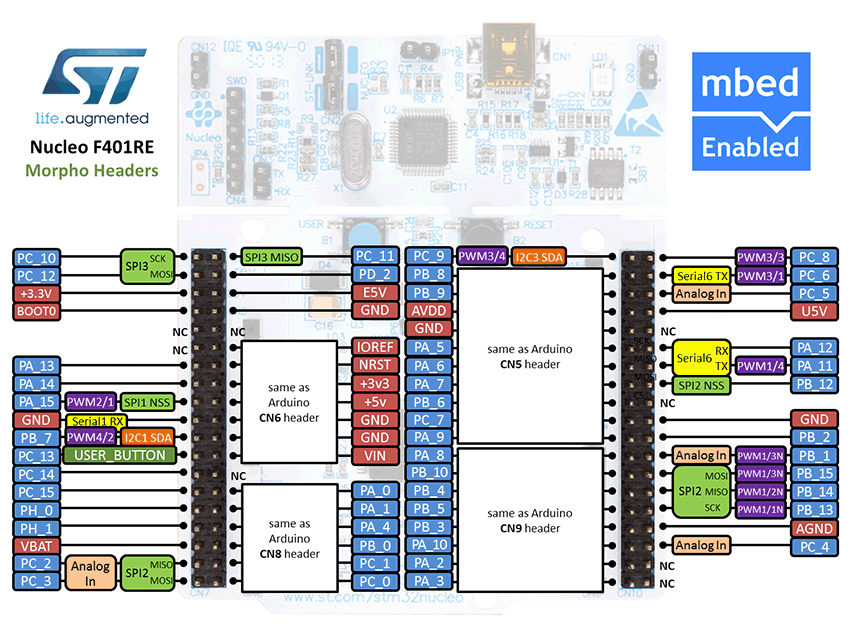
\includegraphics[width=\linewidth]{morpho_pins}
		\end{column}
	\end{columns}
	\begin{block}{Warning}
		You can only use the labels in blue and green!
	\end{block}
	\begin{center}
		\small Full size versions are available at \url{https://mbed.org/platforms/ST-Nucleo-F401RE/}
	\end{center}
\end{frame}

\begin{frame}
	\frametitle{Your Program}
	\begin{columns}[c]
		\begin{column}{0.55\textwidth}
			\lstinputlisting[caption=main.cpp]{code/first_program/2.cpp}
		\end{column}
		\begin{column}{0.45\textwidth}
			\begin{itemize}
				\item Declare a global DigitalOut object
				\item Turn the output on and off in your main loop
			\end{itemize}
			\begin{block}{Note}
				The LED won't seem to be flashing, but it actually is at about 42 MHz, much faster than your eye.
			\end{block}
		\end{column}
	\end{columns}
\end{frame}

\subsection{Waiting}
\label{sub:waiting}
\begin{frame}[fragile]
	\frametitle{Waiting}
	There are three statements that can slow down execution:
	\begin{lstlisting}[numbers=none]
		void wait(float s);
		void wait_ms(int ms);
		void wait_us(int us);
	\end{lstlisting}
	All three will pause execution for the amount of time specified. Use these statements any time you need a controlled delay.
	\begin{block}{Notice}
		Wait and other block statements can have some unintended side effects. This will be demonstrated later.
	\end{block}
\end{frame}

\begin{frame}
	\frametitle{Your Program}
	\begin{columns}[c]
		\begin{column}{0.6\textwidth}
			\lstinputlisting[caption=main.cpp]{code/first_program/3.cpp}
		\end{column}
		\begin{column}{0.4\textwidth}
			\begin{itemize}
				\item Add a wait statement after each write to your output
				\item You should now be able to see your LED flashing
				\item Try making your own patterns!
			\end{itemize}
		\end{column}
	\end{columns}
\end{frame}

\subsection{Compiling}
\label{sub:compiling}
\begin{frame}
	\frametitle{Compiling}
	\begin{columns}[c]
		\begin{column}{0.5\textwidth}
			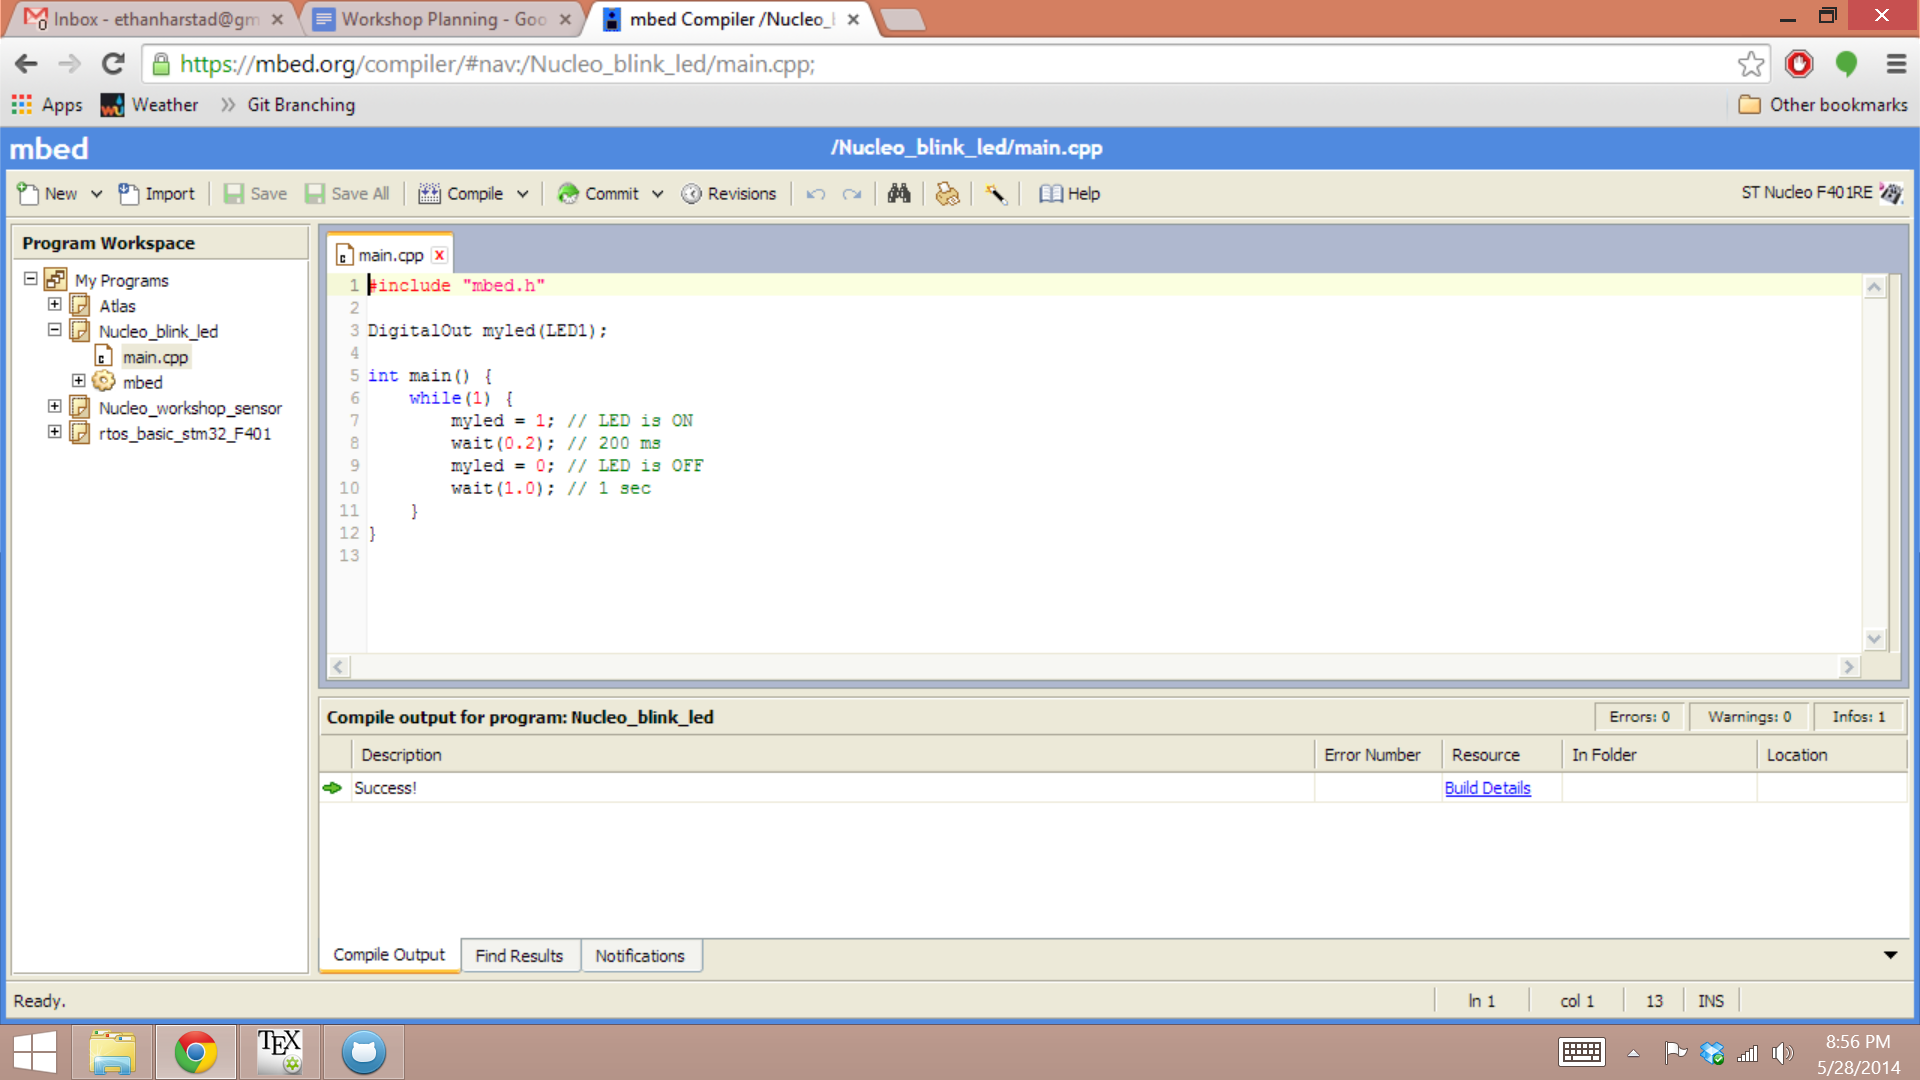
\includegraphics[width=\linewidth]{compile_program}
			\begin{block}{Tip}
				Set your browsers download location to the Nucleo to save time
			\end{block}
		\end{column}
		\begin{column}{0.5\textwidth}
			\begin{enumerate}
				\item Click "Compile" (Ctrl D) to compile your program
				\item A *.bin file will be downloaded
				\item Move the downloaded file to the Nucleo drive
				\item The Nucleo will flash red and green while programming
				\item When the lights stop, your program has started successfully!
			\end{enumerate}
		\end{column}
	\end{columns}
	\begin{center}
		You can also click "Build Only" (Ctrl B) to simply test your code
	\end{center}
\end{frame}